%16/09 - Patricia Álvarez
\chapter{Métodos filogenéticos de inferencia}
Los pasos generales en el proceso de reconstrucción filogenética son: \begin{enumerate}
\item Diseño experimental: selección del ingroup y outgroup, selección de los marcadores moleculares
\item Recolección de datos de secuencia homóloga
\item Ensamblaje de la matriz de secuencias
\item Alineamiento de la secuencia
\item Selección del modelo
\item Inferencia filogenética
\item Construcción del árbol filogenético: soporte estadístico, testar hipótesis filogenética, estimación del tiempo de divergencia
\end{enumerate}

\section{Búsqueda de árboles}
Sólo hay una manera de construir el primer  árbol sin raíz, uno con tres puntas (nodos terminales) y tres ramas. Cada vez que añadimos un taxón, se crean dos ramas. Un árbol con n puntas (taxones) tendrá por tanto 2n-3 ramas.

A partir de unas pocas especies, las búsquedas de árboles sin raíz son exhaustivas y computacionalmente demasiado exigentes. Por ello, se realiza una \textbf{búsqueda heurística}: 
\begin{enumerate}
\item Construir el árbol inicial (Ej., mediante adición secuencial de taxones) y determinar su longitud (ver el número de cambios de un taxón a otro).
\item Construir un conjunto de “árboles vecinos” o alternativos haciendo pequeñas reordenaciones en el árbol inicial, y determinar las longitudes de cada nuevo árbol.
\item Si cualquiera de los árboles vecinos es mejor que el inicial (tienen un menor número de pasos o cambios evolutivos, es decir, la hipótesis se ajusta mejor a los datos): retenerlo y usarlo como punto de partida para una nueva ronda de reordenaciones (es posible que varios de estos árboles sean igual de buenos).
\item Repetir pasos 2 y 3 hasta encontrar un árbol que es mejor que todos sus vecinos.
\item Este árbol es un óptimo local (¡no necesariamente un óptimo global!)
\end{enumerate}

El procedimiento semeja un paseo en un paisaje montañoso, donde nos interesa alcanzar la cumbre más alta (hill climbing).

\begin{figure}[htbp]
\centering
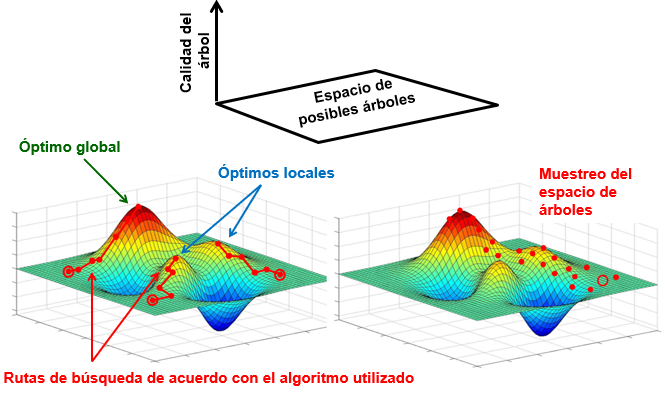
\includegraphics[width=0.7\linewidth]{figs/busqueda-heuristica.png}
\caption{Búsqueda heurística del mejor árbol.}
\end{figure}

Hay varios \textbf{algoritmos de reordenación de ramas (branch swapping)}: \begin{itemize}
\item \textbf{Nearest Neighbour Interchange (NNI):} intercambia dos vecinos por cada rama interna.
\item \textbf{Subtree Pruning and Regrafting (SPR):} se corta un clado (subárbol) y se empalma en todas las ramas del resto del árbol, usando el punto de corte del subárbol como punto de unión. Realmente, NNI es un subconjunto de SPR. 
\item \textbf{Tree Bisection and Reconnection (TBR):} se divide el árbol en dos partes y se reconectan los subárboles usando todos los posibles pares de ramas. NNI y SPR son subsets de TBR.
\end{itemize}

\begin{figure}[htbp]
\centering
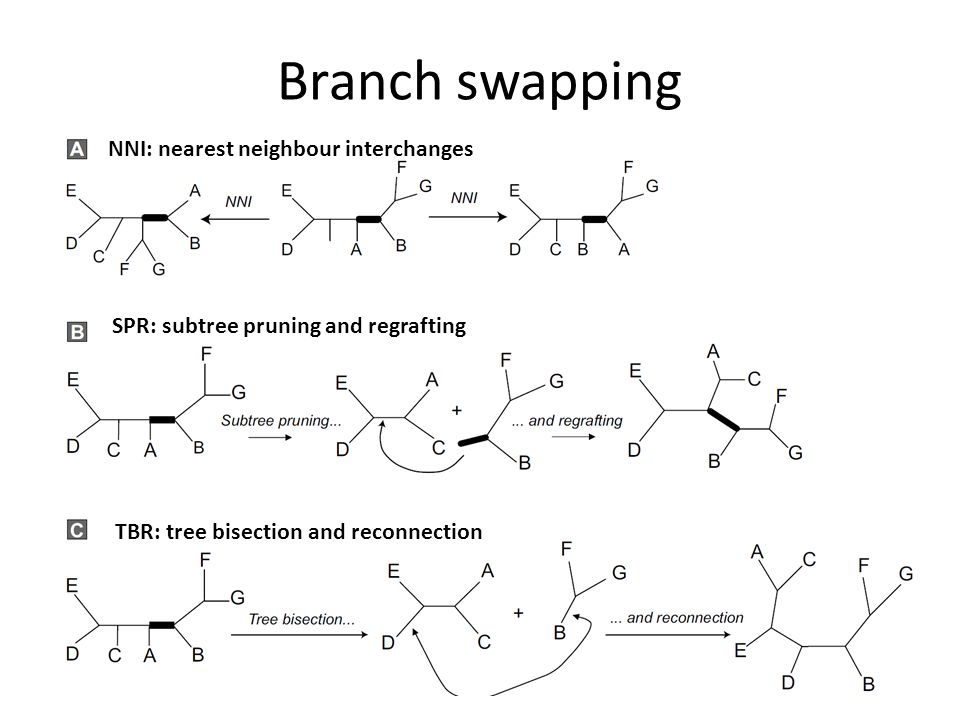
\includegraphics[width=0.7\linewidth]{figs/branch-swapping.jpg}
\caption{Esquemas de los distintos algoritmos de reordenación de ramas.}
\end{figure}

El espacio de árboles puede estar poblado por mínimos locales e islas de árboles óptimos.

\begin{figure}[htbp]
\centering
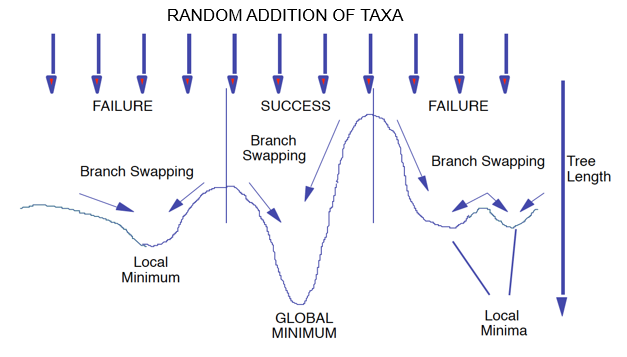
\includegraphics[width=0.7\linewidth]{figs/result-swapping.png}
\caption{Posibles resultados de árboles tras la adición de taxones.}
\end{figure}

\section{Árboles de consenso}
A menudo existen varios árboles candidatos a ser el cladograma más parsimonioso\footnote{véase explicación de parsimonia en el tema 5}. En el siguiente ejemplo, hay tres cladogramas diferentes que son igualmente parsimoniosos para los 4 caracteres estudiados (1-4) en cuatro especies de homínidos. Si aumentamos el número de caracteres y el de taxones, la cantidad de cladogramas igualmente parsimoniosos se dispara y se hace inmanejable. Por lo tanto, es conveniente contar con formas estandarizados de resumir los puntos de acuerdo entre cladogramas rivales para llegar a formar un “árbol de consenso”.

\begin{figure}[htbp]
\centering
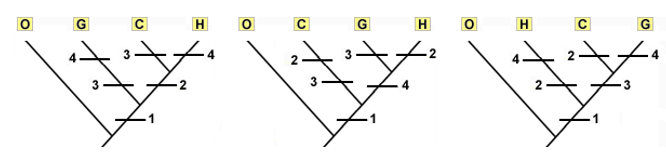
\includegraphics[width=0.7\linewidth]{figs/cladogramas-hominidos.png}
\caption{Tres cladogramas igualmente parsimoniosos de cuatro especies de homínidos: orangutanes, gorilas, chimpancés y humanos.}
\end{figure}

Un árbol de consenso no es otra cosa que un árbol que combina los agrupamientos preferidos a partir de los cladogramas rivales de un determinado grupo de taxones, de tal forma que los agrupamientos discutibles (contenciosos, ambiguos) se condensan en puntos con múltiples ramas (politomías= nodos que portan múltiples ramas). Existen diferentes formas para construir árboles de consenso, pero los tres métodos más comunes son: \begin{itemize}
\item \textbf{Árbol de consenso estricto:} conserva sólo los agrupamientos que comparten todos los cladogramas rivales.
\item \textbf{Árbol de consenso semi-estricto o loose:} conserva todos los agrupamientos que no son contradictorios en los cladogramas rivales.
\item \textbf{Árbol de consenso de regla de la mayoría:} conserva todos los agrupamientos que son apoyados por la mayoría de cladogramas rivales, aunque contradigan a la minoría. Este es el que más se utiliza.
\end{itemize}

\begin{figure}[htbp]
\centering
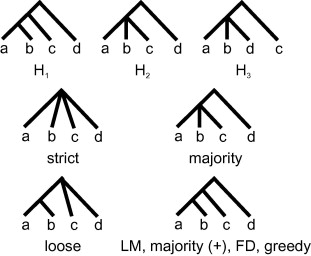
\includegraphics[width=0.5\linewidth]{figs/consensus-trees-types.jpg}
\caption{Distintos tipos de árboles de consenso.}
\end{figure}

Cuando tenemos muchos taxones entre los cuales hay mucha homoplasia, los árboles de consenso estricto van a mostrar gran número de politomías que no pueden resolverse ya que existen conflictos de agrupamiento entre los cladogramas rivales. En esos caso, los árboles de consenso basados en la regla de la mayoría, ofrecen al menos bastantes más hipótesis de trabajo para investigar las relaciones filogenéticas. El ejemplo está basado en más de 70 especies de erizos irregulares; para mayor claridad se han omitido los nombres de las especies. Se estimó que había más de 70.000 cladogramas igualmente parsimoniosos, lo que refleja un gran componente de homoplasia entre los caracteres analizados. El árbol de consenso estricto resultante, ofrece por tanto poca resolución, y la mayoría de los taxones de agrupan en una gran politomía. Por el contrario, el árbol de consenso de regla de la mayoría, resuelve un número de clados mucho mayor que podrán comprobarse en sucesivos análisis. Los valores numéricos para el árbol de consenso de regla de la mayoría miden el porcentaje de cladogramas igualmente parsimoniosos que apoyan cada grupo resuelto.

\begin{figure}[htbp]
\centering
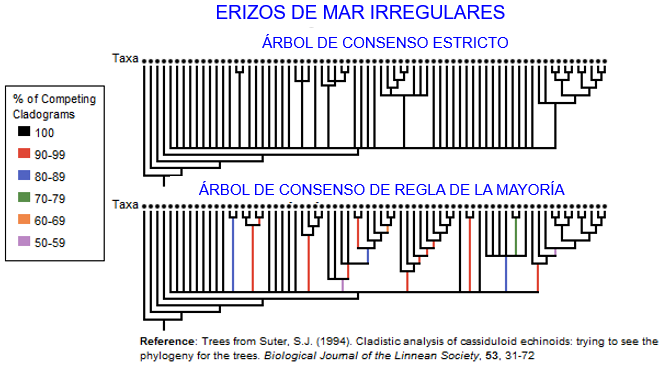
\includegraphics[width=0.7\linewidth]{figs/arbol-erizos.png}
\caption{Árboles filogenéticos de erizos de mar irregulares.}
\end{figure}

\section{Medidas de soporte: confianza en el árbol}
La mayor parte de las medidas científicas van acompañadas de una estima de su precisión del tipo. En el caso de la inferencia filogenética, no es suficiente con estimar hipótesis filogenéticas, sino que es necesario indicar una estima de la confianza que dicha hipótesis presenta. Esto se debe a: 
\begin{itemize}
\item \underline{Error de muestreo:} Nuestros análisis están basados en muestras, pero sólo tenemos una muestra de los datos. Los valores estimados a partir de muestras de una población raramente van a coincidir con el valor real. Una forma de calcular este error es tomando múltiples muestras y comparando las estimas obtenidas entre sí.
\item \underline{Error sistemático:} Asociado a la metodología y las asunciones de los análisis.
\end{itemize}

Las formas de dar apoyo y soporte a un nodo se pueden dar de forma cualitativa (soporte de Bremer), remuestreo (bootstrapping, jackknife) y probabilístico (probabilidad posterior bayesiana): 
\begin{itemize}
\item \textbf{Soporte de Bremer o Decay Index}: se calcula la diferencia en el número de pasos entre el árbol óptimo y el mejor árbol en el que no aparece el clado en cuestión.
\item \textbf{Remuestreo por bootstrapping:} se remuestrean los caracteres al azar con reemplazamiento múltiples veces. Se realiza el análisis con cada nueva pseudoréplica utilizando los mismos parámetros que en el análisis original. Se analiza la coincidencia entre las topologías obtenidas resumiéndolas en un majority-rule consensus tree. Las pseudoréplicas se construyen a partir de la matriz original con reemplazamiento para construir una nueva matriz del mismo tamaño que la original. La frecuencia con que aparece un determinado grupo es una medida de la estabilidad de ese grupo. Estos valores se muestran en un árbol de majority-rule consensus y se da información adicional en una tabla (de biparticiones). Los valores de bootstrap son conservadores; son un índice relativo del soporte estadístico de los grupos, proporcionado por los datos que se están analizando bajo un método de análisis concreto: valores altos de bootstrap nos indican la existencia de una señal filogenética “fuerte” en los datos. Estudios realizados con datos empíricos y simulaciones han indicado que un 70\% de soporte de bootstrap puede considerarse apoyo razonable para una relación determinada. No obstante, este número se puede modificar según se necesite.
\item \textbf{Remuestreo por Jackknife:} Jackknife es muy similar al bootstrap, sólo se diferencia en la estrategia de remuestreo de los caracteres. Una cierta proporción de los caracteres es eliminada al azar (por ej.: 50\%). No hay reemplazo, por lo que la matriz es más pequeña. Se analizan las pseudoréplicas y los resultados se resumen en un majority-rule consensus tree. Jackknifing y bootstrapping suelen dar resultados similares y se interpretan de forma similar. Jackknife se está utilizando cada vez menos y se está reemplazando por bootstrap al estar reduciendo los datos.
\end{itemize}

\begin{figure}[htbp]
\centering
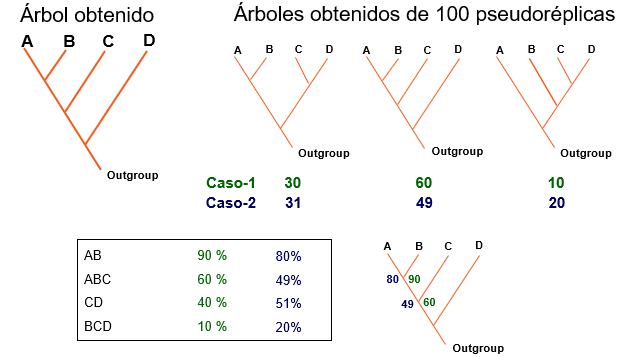
\includegraphics[width=0.7\linewidth]{figs/ejemplos-bootstrap.png}
\caption{Ejemplos del cálculo de bootstrap. En el primer caso (mostrado en verde), tras 100 pseudoréplicas, han salido tres árboles con frecuencias de 30, 60 y 10. Tanto en el primer como en el segundo árbol, los taxones A y B se han relacionado juntos, por lo que esa dicotomía tiene un soporte de bootstrap de 90 (60 + 30). La siguiente relación más soportada, con un bootstrap de 60, es la de relacionar el taxón C con el antepasado común de A y B, por lo que el árbol final muestra esa variante (la otra opción sería relacionar C con D, como hacen los otros dos árboles, pero su frecuencia es de 40). En el segundo caso (mostrado en azul), las frecuencias han cambiado. Ahora, la relación de A y B pasa a tener un soporte de 80 (31 + 49), y así sucesivamente.}
\end{figure}
